\subsection[\texorpdfstring{$\textup{N}^3\textup{LO} + \textup{N}^3\textup{LL}$ in the HTL}{N3LO + N3LL in the HTL}]{\texorpdfstring{\boldmath$\textup{N}^3\textup{LO} + \textup{N}^3\textup{LL}$ in the HTL}{N3LO + N3LL in the HTL}}

%\textit{Authors:} Ajjath A H, Hua-Sheng Shao (2209.03914)

\textbf{Ajjath A H, Hua-Sheng Shao~\cite{Ajjath:2022kpv}.}

\noindent Theoretical predictions for the Higgs boson pair production cross section can be further improved by resumming threshold logarithms from soft-gluon emissions. In this subsection, these logarithms are resummed to N$^3$LL accuracy~\cite{Ajjath:2022kpv}, following the formalism outlined briefly below.

Within the QCD-improved parton model, the differential cross section in the invariant mass squared $m_{hh}^2$
of the Higgs boson pair, for hadronic collisions at the centre-of-mass energy $\sqrt{s}$, can be written as a convolution of the partonic flux $\phi_{ab}$ and the perturbative coefficient function $\Delta_{ab\to hh}$
\begin{equation}\label{eq:partonmodel}
    m_{hh}^2 \dfrac{d}{d m_{hh}^2}\sigma_{pp\rightarrow hh}(s,m_{hh}^2) = \tau \sum_{a,b=q,\bar q,g} \int_\tau^1 \frac{dz}{z} \phi_{ab}\left(\frac{\tau}{z},\mu_F^2\right)~ \Delta_{ab\rightarrow hh}  \left(z,m_{hh}^2,\mu_F^2\right)\,,
\end{equation}
where $\tau\equiv m_{hh}^2/s$, $z\equiv m_{hh}^2/\hat{s}$, with $\sqrt{\hat{s}}$
the partonic centre-of-mass energy.

 In the threshold limit, $z\rightarrow1$, the dominant (leading-power, LP) terms arise from both virtual loop corrections and soft, unresolved real-gluon emissions. These contributions take the form of Dirac delta functions, $\delta(1-z)$,  and plus-distributions, such as $ {\cal D}_k(z) \equiv  \left(\frac{\ln^k{(1-z)}}{1-z}\right)_+$, reflecting the incomplete cancellation between virtual and real radiation associated with soft-gluon emissions. These singular threshold contributions can be systematically factorized as
\begin{align}\label{eq:partonicxsec}
    \Delta^{\text{LP}}_{gg\rightarrow hh}(z,m_{hh}^2,\mu_F^2) =& H_{gg\rightarrow hh}(m_{hh}^2,\mu_R^2) ~\delta(1-z)\otimes S_{\Gamma,gg}(z,m_{hh}^2,\mu_F^2,\mu_R^2)\,,
\end{align}
where $H_{gg\rightarrow hh}$ encodes the process-dependent hard virtual corrections after infrared-divergence subtraction, and
 $S_{\Gamma,gg}$
  is the soft-collinear function describing gluon emissions that are soft, collinear, or both with respect to the parent partons. Singular terms are retained in this factorization, while power-suppressed corrections in $(1-z)$ are neglected. The threshold-enhanced logarithms resummed in this approach are universal and can largely be expressed in terms of process-independent anomalous dimensions and splitting functions. Detailed structures of these functions are given in Refs.~\cite{Ravindran:2005vv,Ahmed:2020nci,Ajjath:2022kpv}.

The universal nature of the soft and collinear terms allows the resummation of large logarithms to all orders in $\alpha_s$ using renormalization group methods. This resummation is efficiently performed in Mellin $N$-moment space, where the threshold limit $z\rightarrow 1$ corresponds to $N\rightarrow \infty$:
\begin{align}
    \Delta_{gg\rightarrow hh}^{\rm res}(N,m_{hh}^2,\mu_F^2) =&  \int_0^1 dz ~z^{N-1}\Delta^{\text{LP}}_{gg\rightarrow hh}\left(z,m_{hh}^2,\mu_F^2\right)
    \nonumber \\
    =  g_{0,gg\to hh}(m_{hh}^2,\mu_F^2,\mu_R^2)
    & 
    ~\exp \left(\tilde{C}_{0,gg} (a_s(\mu_R^2)) + g_{1,gg} (\omega)\ln N + \sum_{k=2}{a_s^{k-2}(\mu_R^2)~g_{k,gg} (\omega)}\right)\,,
    \label{DeltaN}
\end{align}
where $a_s\equiv \alpha_s/4\pi$ and $\omega \equiv 2 \beta_0 a_s(\mu_R^2) \ln N$. The factor $g_{0,gg\to hh}$, outside the exponent, arises from the $N$-independent hard function and the Altarelli-Parisi splitting kernels, while the functions $g_{k,gg}$, $k\ge 1$, encode the resummation of logarithmic contributions up to the specified logarithmic accuracy (LL, NLL, NNLL, N$^3$LL, etc.).
Furthermore, the exponent contains an additional $N$-independent coefficient, $\tilde{C}_{0,gg}$, arising from the ${\cal O}(1)$ terms of ${\cal D}_k(z)$ after the Mellin transform; it depends on the Riemann zeta functions $\zeta_n$ and the Euler-Mascheroni constant $\gamma_E$. 

The structure above ensures that the resummation captures all LP threshold logarithms at each order, resulting in a perturbative series with greatly improved convergence and reduced dependence on the renormalization and factorization scales. Matching to fixed-order calculations guarantees the exact reproduction of known results and prevents double counting of terms already included at a given order. At the $\NkLONkLL$ accuracy, the double counting corresponds to $\Delta^{\text{LP}}_{gg\to hh}$ expanded up to N$^k$LO in $\alpha_s$. However, at a given logarithmic accuracy, the right-hand side of the resummation formalism in Eq.~\eqref{DeltaN} is not uniquely defined. The assignment of $N$-independent terms inside or outside the exponent introduces a degree of arbitrariness, referred to as the resummation scheme dependence~\cite{Ajjath:2022kpv}. Four different resummation schemes, denoted ${\rm N_1}$, $\rm{\overline N}_1$, ${\rm N_2}$, and $\rm{\overline N}_2$, are considered in Ref.~\cite{Ajjath:2022kpv} (see their definitions in Section 2.4 of that reference).

A comparison of inclusive Higgs boson pair cross sections at $\sqrt{s}=14$ TeV in the HTL, at several perturbative orders and in different resummation schemes, is shown in Fig.~\ref{fig:Verical_prescription}. Both the fixed-order N$^k$LO and resummation-improved N$^k$LO+N$^k$LL predictions are presented, with error bars indicating scale uncertainties. We stress a few key points:
\begin{itemize}
    \item Although a significant resummation scheme dependence is observed at NLO+NLL, this dependence decreases as higher orders are included and becomes moderate at N$^3$LO+N$^3$LL.
    \item The results in the $\ResNTwo$ and $\ResNbTwo$ schemes show faster perturbative convergence than those in the other two schemes.
    \item The inclusion of threshold resummation further reduces scale uncertainties. For instance, in the $\ResNbTwo$ scheme, the N$^3$LO+N$^3$LL scale-uncertainty band is reduced by a factor of two compared to the N$^3$LO result, and nearly by a factor of four compared to the NNLO+NNLL result in the same scheme.
    \item The resummation scheme uncertainty at N$^3$LO+N$^3$LL is subdominant compared to the residual scale uncertainty. At $14$ TeV, for example, we have \begin{equation*}\sigma_{\rm N^3LO+N^3LL}=38.70\left(^{+0.85\%}_{-0.87\%}\right)_{\rm scale}\left(^{+0.08\%}_{-0.39\%}\right)_{\rm scheme}~\mathrm{fb}.
    \end{equation*}
\end{itemize}
Therefore, in the following, we consider the $\ResNbTwo$ scheme only. Table~\ref{tab:ResumN3LON3LLinclusivexs} summarizes inclusive cross sections, from NLO+NLL to N$^3$LO+N$^3$LL, in the HTL at $\sqrt{s}=14$ TeV. Inclusion of N$^3$LL resummation corrections increases the N$^3$LO cross section by around $1\%$ and reduces the scale uncertainty by about a factor of two.


\begin{figure*}[ht]
\centering
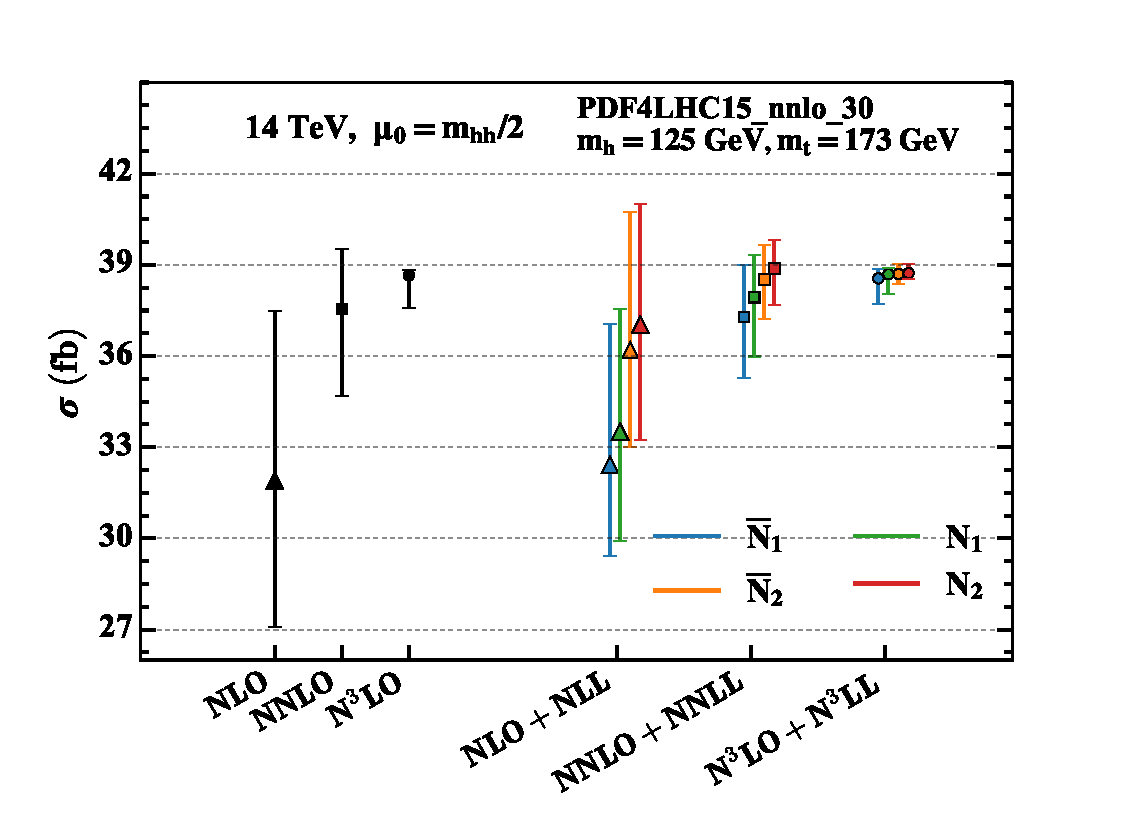
\includegraphics[width=0.5\textwidth]{N3LO_QCD_SM/N3LO_N3LL/Images/prescription_14TeV_YR5.pdf}
\caption{Inclusive Higgs boson pair cross sections at $\sqrt{s}=14~\textup{TeV}$ in the HTL at several perturbative orders and in different resummation schemes. The error bars indicate scale uncertainties. Results shown are from Ref.~\cite{Ajjath:2022kpv}.}
\label{fig:Verical_prescription}
\end{figure*}

\begin{table}[htbp] 
\begin{center}
\newcolumntype{P}[1]{>{\centering\arraybackslash}p{#1}}
{\renewcommand{\arraystretch}{1.5}
%\begin{tabular}{|P{2.5cm}|P{2.5cm}|P{2.5cm}|}
\begin{tabular}{P{2.6cm}P{2.6cm}P{2.6cm}}
%\hline
    \toprule
    $\sigma_{\textup{NLO}+\textup{NLL}}$ $[\textup{fb}]$
    & $\sigma_{\textup{NNLO}+\textup{NNLL}}$ $[\textup{fb}]$
    & $\sigma_{\textup{N}^3\textup{LO}+\textup{N}^3\textup{LL}}$ $[\textup{fb}]$
    \\
%  \hline
    \midrule
  $36.19^{+12.5\%}_{-8.8\%}$ &
  $38.52^{+3.0\%}_{-3.4\%}$ &
 $38.70_{-0.85\%}^{+0.87\%}$
 \\
% \hline
    \bottomrule
\end{tabular}}
%\end{small}
\caption{Soft-gluon resummation–improved inclusive cross sections in the HTL at $\sqrt{s}=14~\textup{TeV}$. The quoted uncertainties correspond to $7$-point scale variations. Only results in the $\ResNbTwo$ scheme are shown.}
\label{tab:ResumN3LON3LLinclusivexs}
\end{center}
\end{table}

\begin{figure*}[!htbp]
\centering
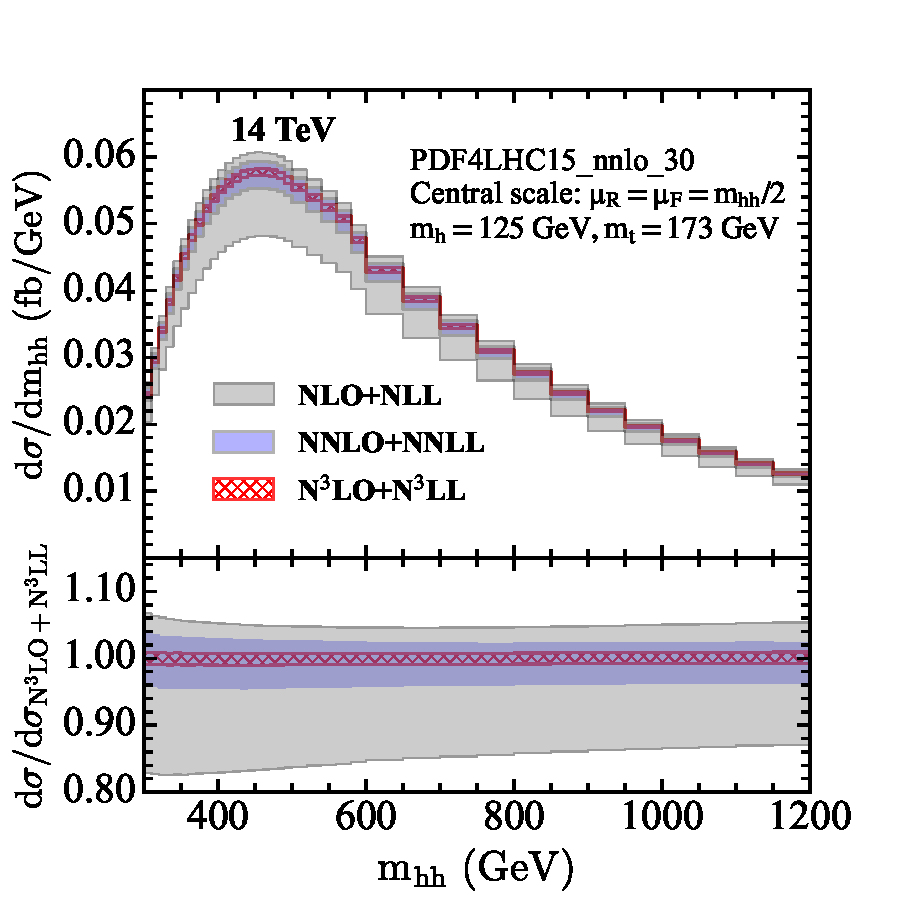
\includegraphics[width=0.5\textwidth]{N3LO_QCD_SM/N3LO_N3LL/Images/diff_large_mt_13_14_resum_CERNYR5.pdf}
\\
\caption{Inclusive invariant-mass distributions for Higgs boson pair production at $\sqrt{s}=14$ TeV in the HTL, from NLO+NLL to N$^3$LO+N$^3$LL. The error bands correspond to $7$-point scale variations. Results shown are from Ref.~\cite{Ajjath:2022kpv}.}
\label{fig:xs_vs_mhh_Res_N3LON3LL}
\end{figure*}

The differential prediction for the Higgs boson pair invariant mass $m_{hh}$ in Fig.~\ref{fig:xs_vs_mhh_Res_N3LON3LL} further demonstrates the perturbative convergence of the strong-coupling expansion. Soft-gluon resummation induces only a modest shift in the spectrum and further reduces the fractional scale errors.
